\clearpage
\section{Mô phỏng tác vụ hàn đơn giản}
Xét một đường hàn góc thẳng trên phôi chữ T. Robot SR5 phải đưa đầu mỏ từ đầu \(A\) đến đầu \(B\), giữ nguyên hướng mỏ và khoảng cách đến đường hàn. Bài thử bắt đầu tại tư thế hàn đầu tiên và kết thúc ở tư thế hàn cuối cùng. Chương trình mô phỏng chuyển động của robot trong ROS~2 bằng MoveIt~2 và bộ giải KDL.

\subsection{Điều kiện đầu vào và quỹ đạo đặt}
Phôi \texttt{coupon\_tee} được tạo bằng bộ sinh hình học của Weldment Dataset với hạt giống 42. Cạnh số 10 là giao tuyến thẳng giữa hai mặt cần hàn. Hệ phôi có cùng hướng trục với hệ thế giới và gốc đặt tại \((500,0,300)\,\mathrm{mm}\). Đế robot gắn cố định tại gốc thế giới. Với tọa độ tính bằng milimét trong hệ đế, hai đầu đường hàn và chiều dài của cạnh là
\[
  A=(497{,}925,-58{,}700,300),\qquad B=(497{,}925,58{,}700,300),
  \qquad L=\|B-A\|=117{,}4\,\mathrm{mm}.
\]
Chọn trục \(x\) của đầu mỏ theo tiếp tuyến \(\mathbf x_d=(B-A)/L\). Trục \(z\) của mỏ hướng từ mặt bích về phía đường hàn. Chương trình lấy hướng ngược với tổng hai pháp tuyến đơn vị của hai mặt phôi, loại thành phần dọc tiếp tuyến rồi chuẩn hóa. Trên cạnh đã chọn, \(\mathbf z_d\simeq(0{,}605972,0,-0{,}795486)^{\mathsf T}\). Hướng đặt giữ cố định suốt đoạn thẳng:
\[
  R_d=[\,\mathbf x_d\quad\mathbf z_d\times\mathbf x_d\quad\mathbf z_d\,].
\]
Để TCP cách đường hàn \(h=5\,\mathrm{mm}\) dọc trục mỏ, hai vị trí đích của TCP là \(\mathbf p_A=A-h\mathbf z_d\) và \(\mathbf p_B=B-h\mathbf z_d\). Do đó TCP di chuyển theo chiều \(+y\) từ \(-58{,}700\) đến \(58{,}700\,\mathrm{mm}\), với \(x\simeq494{,}895\,\mathrm{mm}\) và \(z\simeq303{,}977\,\mathrm{mm}\).

Để vận tốc và gia tốc bằng không tại hai đầu, sử dụng luật tiến trình bậc năm. Với \(u=t/T\), ta có
\begin{align}
 s(u)&=10u^3-15u^4+6u^5,\qquad 0\le u\le1,\\
 \mathbf p_d(t)&=\mathbf p_A+s(u)(\mathbf p_B-\mathbf p_A),\\
 v_d(t)&=\|\dot{\mathbf p}_d(t)\|=\frac{30L}{T}u^2(1-u)^2 .
\end{align}
Tại \(u=1/2\), vận tốc đạt cực đại \(1{,}875L/T\). Chọn tốc độ đỉnh \(5\,\mathrm{mm/s}\) suy ra \(T=44{,}025\,\mathrm{s}\). Chia đều khoảng \([0,T]\) thành 881 khoảng, thu được 882 pose đặt với \(t_k=kT/881\), \(k=0,\ldots,881\). Mỗi pose truyền cho MoveIt~2 gồm vị trí tính bằng mét và hướng \(R_d\). Mô hình dụng cụ đã chứa đoạn từ mặt bích đến TCP dài \(180\,\mathrm{mm}\).

\subsection{Giải động học nghịch cho từng mẫu}
Tại thời điểm \(t_k\), đích \(T_{d,k}\) được giữ cố định trong suốt các vòng lặp IK. Sau khi nghiệm được chấp nhận, chương trình mới chuyển sang \(t_{k+1}\). Các bước áp dụng mục 2.2.2 như sau.
\begin{enumerate}
  \item \textbf{Khởi tạo.} Ở mẫu đầu, thử các cấu hình ban đầu cho nhóm sáu khớp \texttt{rokae\_arm}. Với \(k>0\), lấy \(\mathbf q_k^{(0)}=\mathbf q_{k-1}^{\star}\). Lệnh \texttt{setFromIK} nhận đích của \texttt{welding\_tcp} và thời gian tìm kiếm \(0{,}05\,\mathrm{s}\) cho các mẫu tiếp theo.
  \item \textbf{Tính sai số và bước Newton.} Tại vòng \(j\), KDL tính FK, lập sai số \(\mathbf e_k^{(j)}\) theo \eqref{eq:sr5-ik-error} và tính Jacobi hình học tại TCP. KDL giải \(J_{\mathrm{TCP}}\Delta\mathbf q\simeq\mathbf e_k^{(j)}\) bằng SVD có trọng số theo \eqref{eq:sr5-ik-kdl}. Bộ giải cộng bước hiệu chỉnh vào góc khớp sau khi xử lý giới hạn khớp. Nếu sai số tăng, thuật toán quay lại cấu hình trước và giảm bước.
  \item \textbf{Dừng và chọn nghiệm.} Ở chế độ giải đủ vị trí và hướng, KDL kiểm tra riêng chuẩn của phần tịnh tiến (m) và phần quay (rad) với cùng ngưỡng số mặc định \(10^{-5}\). Một lần thử có tối đa 500 vòng lặp. Khi cần, bộ giải có thể thử cấu hình khởi tạo khác trong thời gian tìm kiếm. Hàm kiểm tra của ứng dụng chỉ chấp nhận cấu hình thỏa giới hạn khớp và qua kiểm tra va chạm với mô hình robot, bàn và phôi. Nếu \(\|\mathbf q_k^\star-\mathbf q_{k-1}^\star\|_\infty>0{,}05\,\mathrm{rad}\), chương trình dừng để tránh chuyển nhánh đột ngột.
\end{enumerate}

\noindent\textbf{Ví dụ tính bước từ mẫu 440 sang mẫu 441.}
Tại hai mẫu giữa đường, thời điểm tương ứng là \(21{,}98751\) và \(22{,}03749\,\mathrm{s}\). Tọa độ \(y\) đặt của TCP tăng từ \(-0{,}124929\) lên \(+0{,}124929\,\mathrm{mm}\). Thay nghiệm mẫu 440 vào FK, so với đích mẫu 441, sai số vị trí ban đầu xấp xỉ \((0{,}000060,0{,}249918,-0{,}000009)\,\mathrm{mm}\). Với trọng số đơn vị tại bước này, lấy Jacobi đã lưu ở mẫu 440 và tính \(J^+\mathbf e\) thu được
\[
  \Delta\mathbf q\simeq10^{-3}
    [0{,}57766,\;0{,}04580,\;-0{,}19885,\;-0{,}84323,\;0{,}03976,\;1{,}27599]^{\mathsf T}
    \,\mathrm{rad}.
\]
Bước tính lại từ dữ liệu FK và Jacobi khớp với hiệu \(\mathbf q_{441}^{\star}-\mathbf q_{440}^{\star}\) trong quỹ đạo đã ghi. Sau hiệu chỉnh, sai số vị trí của mẫu 441 còn khoảng \(0{,}000086\,\mathrm{mm}\).

\subsection{Đầu ra và kiểm chứng}
Đầu ra chính là 882 dòng \((t_k,q_{1,k},\ldots,q_{6,k})\) trong \texttt{trajectory.csv}, với góc khớp theo quy ước URDF, tính bằng radian. Ba cấu hình sau cho thấy sự thay đổi của cả sáu khớp khi TCP di chuyển theo một đường thẳng.
\begin{center}
\small
\begin{tabular}{@{}rrrrrrrr@{}}
\toprule
\(k\)&\(t_k\) (s)&\(q_1\)&\(q_2\)&\(q_3\)&\(q_4\)&\(q_5\)&\(q_6\)\\
\midrule
0   &0       &2,64076&$-0{,}03260$&2,15381&$-2{,}43737$&$-0{,}46610$&0,51094\\
441 &22,03749&2,77247&$-0{,}00927$&2,13097&$-2{,}60220$&$-0{,}43971$&0,77584\\
881 &44,025  &2,91667&$-0{,}01211$&2,06013&$-2{,}82577$&$-0{,}45018$&1,10464\\
\bottomrule
\end{tabular}
\end{center}
Vị trí và hướng được kiểm tra lại bằng FK tại từng mẫu. Sai số vị trí lớn nhất là \(0{,}009993\,\mathrm{mm}\), sai số hướng lớn nhất là \(4{,}60\times10^{-5}\) độ. Tốc độ TCP đỉnh tính từ \(\|J_v\dot{\mathbf q}\|\) đạt \(4{,}99997\,\mathrm{mm/s}\), với \(\dot{\mathbf q}\) ước lượng bằng sai phân theo thời gian. Bước góc khớp lớn nhất giữa hai mẫu là \(0{,}07462^\circ\). Trên 5\,286 lượt kiểm tra các cấu hình nội suy, chương trình ghi nhận 0 lượt va chạm và 0 lượt vượt giới hạn góc khớp.
\begin{figure}[H]
  \centering
  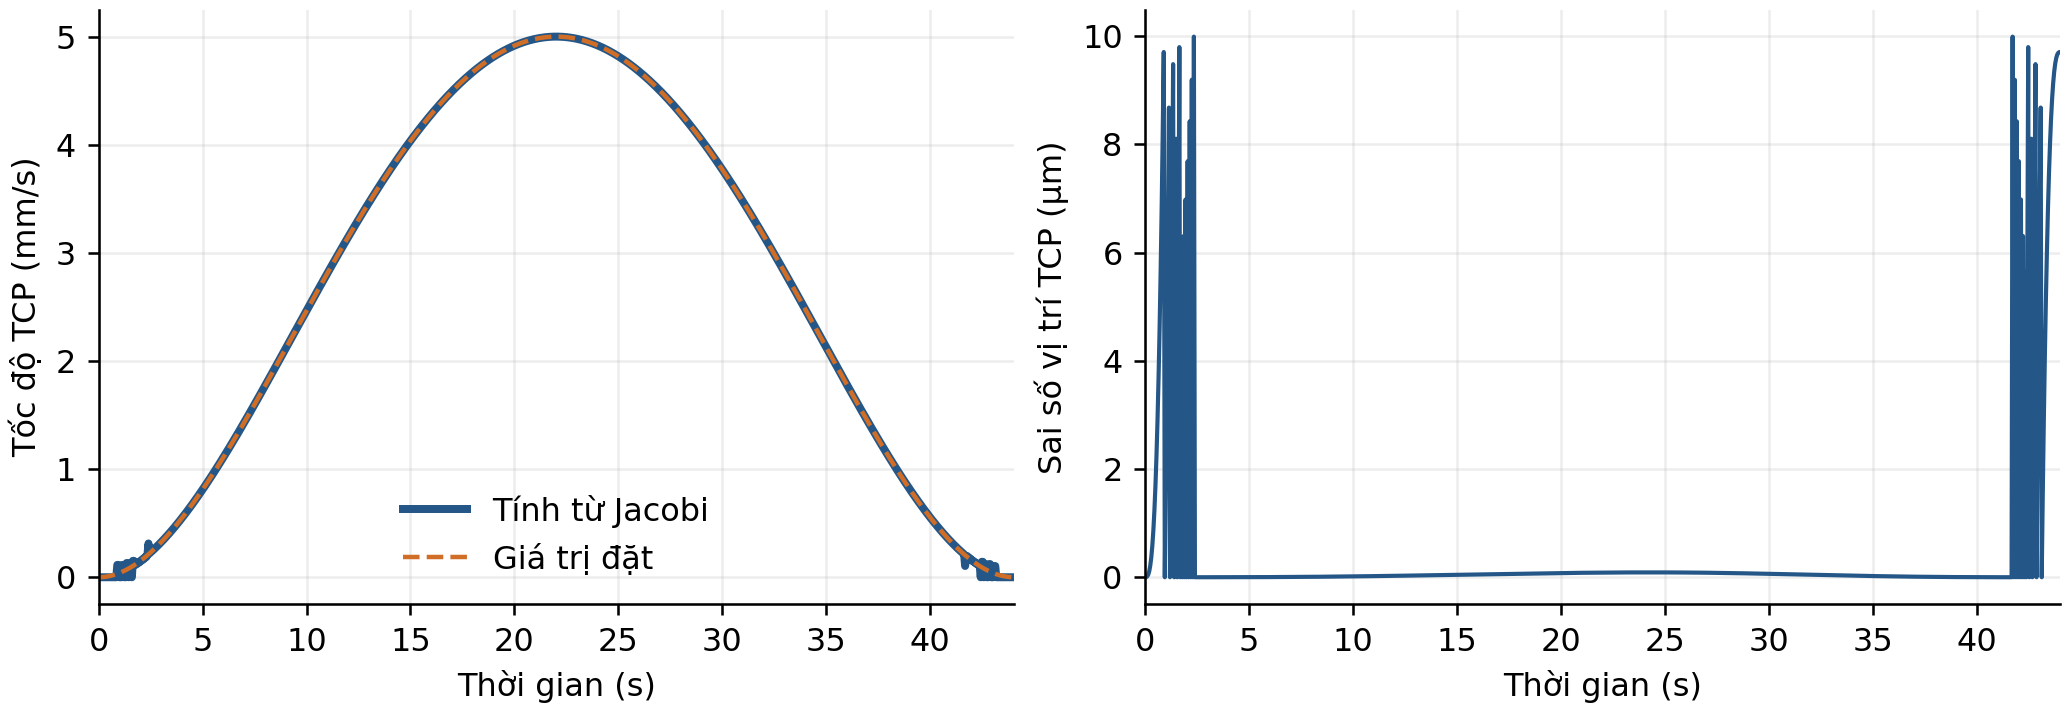
\includegraphics[width=.94\linewidth]{hinh/03-mo-phong/3.3-han-thang/hinh-3-3-quy-dao.png}
  \caption{Tốc độ đầu mỏ và sai số vị trí dọc theo đường hàn thẳng, tính từ kết quả mô phỏng}
  \label{fig:sr5-straight-speed}
\end{figure}
